%% LyX 2.0.3 created this file.  For more info, see http://www.lyx.org/.
%% Do not edit unless you really know what you are doing.
\documentclass[10pt]{beamer}\usepackage[]{graphicx}\usepackage[]{color}
%% maxwidth is the original width if it is less than linewidth
%% otherwise use linewidth (to make sure the graphics do not exceed the margin)
\makeatletter
\def\maxwidth{ %
  \ifdim\Gin@nat@width>\linewidth
    \linewidth
  \else
    \Gin@nat@width
  \fi
}
\makeatother

\definecolor{fgcolor}{rgb}{0.345, 0.345, 0.345}
\newcommand{\hlnum}[1]{\textcolor[rgb]{0.686,0.059,0.569}{#1}}%
\newcommand{\hlstr}[1]{\textcolor[rgb]{0.192,0.494,0.8}{#1}}%
\newcommand{\hlcom}[1]{\textcolor[rgb]{0.678,0.584,0.686}{\textit{#1}}}%
\newcommand{\hlopt}[1]{\textcolor[rgb]{0,0,0}{#1}}%
\newcommand{\hlstd}[1]{\textcolor[rgb]{0.345,0.345,0.345}{#1}}%
\newcommand{\hlkwa}[1]{\textcolor[rgb]{0.161,0.373,0.58}{\textbf{#1}}}%
\newcommand{\hlkwb}[1]{\textcolor[rgb]{0.69,0.353,0.396}{#1}}%
\newcommand{\hlkwc}[1]{\textcolor[rgb]{0.333,0.667,0.333}{#1}}%
\newcommand{\hlkwd}[1]{\textcolor[rgb]{0.737,0.353,0.396}{\textbf{#1}}}%
\newcommand\myeq{\stackrel{\mathclap{\normalfont\mbox{d}}}{=}}




\usepackage{fontawesome5}
\usepackage{framed}
\makeatletter
\newenvironment{kframe}{%
 \def\at@end@of@kframe{}%
 \ifinner\ifhmode%
  \def\at@end@of@kframe{\end{minipage}}%
  \begin{minipage}{\columnwidth}%
 \fi\fi%
 \def\FrameCommand##1{\hskip\@totalleftmargin \hskip-\fboxsep
 \colorbox{shadecolor}{##1}\hskip-\fboxsep
     % There is no \\@totalrightmargin, so:
     \hskip-\linewidth \hskip-\@totalleftmargin \hskip\columnwidth}%
 \MakeFramed {\advance\hsize-\width
   \@totalleftmargin\z@ \linewidth\hsize
   \@setminipage}}%
 {\par\unskip\endMakeFramed%
 \at@end@of@kframe}
\makeatother

\definecolor{shadecolor}{rgb}{.97, .97, .97}
\definecolor{messagecolor}{rgb}{0, 0, 0}
\definecolor{warningcolor}{rgb}{1, 0, 1}
\definecolor{errorcolor}{rgb}{1, 0, 0}
\newenvironment{knitrout}{}{} % an empty environment to be redefined in TeX

\usepackage{alltt}
\usepackage[T1]{fontenc}
\setcounter{secnumdepth}{3}
\setcounter{tocdepth}{3}
\usepackage{tikz}
\usepackage{color}
\usepackage{colortbl}
\usepackage{dcolumn}
\usepackage{amsmath}
\usepackage{tikz}
\usepackage{floatflt}
\usepackage{multicol}
\usepackage{multirow}
\usepackage{listings}
\usepackage{tabularx}
\usepackage{amssymb}% http://ctan.org/pkg/amssymb
\usepackage{pifont}% http://ctan.org/pkg/pifont
\usepackage{bbm}
\usepackage{siunitx}
\usepackage{url}
\usepackage{verbatim}
\usepackage{enumerate}
\usepackage{algorithmic}
\usepackage{algorithm}
\usepackage[flushleft]{threeparttable}
\usepackage{algorithm}
\usepackage{amsfonts}
\usepackage{booktabs}
\usepackage{siunitx}

\usepackage{hyperref}
\hypersetup{
    colorlinks=magenta,
    linkcolor=blue,
    filecolor=magenta,      
    urlcolor=magenta
     }
     
    \definecolor{links}{HTML}{2A1B81}
\hypersetup{colorlinks,linkcolor=blue, urlcolor=magenta}


\makeatletter

%%%%%%%%%%%%%%%%%%%%%%%%%%%%%% LyX specific LaTeX commands.
\providecommand{\LyX}{\texorpdfstring%
  {L\kern-.1667em\lower.25em\hbox{Y}\kern-.125emX\@}
  {LyX}}


%%%%%%%%%%%%%%%%%%%%%%%%%%%%%% Textclass specific LaTeX commands.
 % this default might be overridden by plain title style
 \newcommand\makebeamertitle{\frame{\maketitle}}%
 \AtBeginDocument{
   \let\origtableofcontents=\tableofcontents
   \def\tableofcontents{\@ifnextchar[{\origtableofcontents}{\gobbletableofcontents}}
   \def\gobbletableofcontents#1{\origtableofcontents}
 }
 \def\lyxframeend{} % In case there is a superfluous frame end
 \long\def\lyxframe#1{\@lyxframe#1\@lyxframestop}%
 \def\@lyxframe{\@ifnextchar<{\@@lyxframe}{\@@lyxframe<*>}}%
 \def\@@lyxframe<#1>{\@ifnextchar[{\@@@lyxframe<#1>}{\@@@lyxframe<#1>[]}}
 \def\@@@lyxframe<#1>[{\@ifnextchar<{\@@@@@lyxframe<#1>[}{\@@@@lyxframe<#1>[<*>][}}
 \def\@@@@@lyxframe<#1>[#2]{\@ifnextchar[{\@@@@lyxframe<#1>[#2]}{\@@@@lyxframe<#1>[#2][]}}
 \long\def\@@@@lyxframe<#1>[#2][#3]#4\@lyxframestop#5\lyxframeend{%
   \frame<#1>[#2][#3]{\frametitle{#4}#5}}

\renewcommand{\footnotesize}{\fontsize{6pt}{6pt}\selectfont}


\newcommand{\indep}{\rotatebox[origin=c]{90}{$\models$}}

% https://dkumor.com/posts/technical/2018/08/15/causal-tikz/

% Tikz settings optimized for causal graphs.
% Just copy-paste this part
\usetikzlibrary{shapes,decorations,arrows,calc,arrows.meta,fit,positioning}
\tikzset{
    -Latex,auto,node distance =1 cm and 1 cm,semithick,
    state/.style ={ellipse, draw, minimum width = 0.7 cm},
    point/.style = {circle, draw, inner sep=0.04cm,fill,node contents={}},
    bidirected/.style={Latex-Latex,dashed},
    el/.style = {inner sep=2pt, align=left, sloped}
}


%%%%%%%%%%%%%%%%%%%%%%%%%%%%%% User specified LaTeX commands.
%\usetheme{Warsaw}
\usetheme{Boadilla}
%\setbeamertemplate{navigation symbols}{}
%gets rid of bottom navigation bars
%\setbeamertemplate{footline}[page number]{}
%\setcounter{page}{44}
%\setbeamertemplate{footline}{}


\makeatother
\IfFileExists{upquote.sty}{\usepackage{upquote}}{}

\begin{document}


\title[OOD Generalization of Uplift Models]{Out-of-Distribution Generalization of Uplift Models}
\author[Leo Guelman]{Leo Guelman}
\institute[RBC Royal Bank]{Head Statistician | Royal Bank of Canada}
\date[September 2022]
{ECML 2022 \\  Uplift Modeling Workshop}
\makebeamertitle

\lyxframeend{}


%%%%Slide

\begin{frame}
[fragile]\frametitle{Introduction}

\begin{itemize} 

\item  Most uplift modeling methods assume i.i.d. data.

\vskip2pt

\item In most practical settings this assumption is violated:

\vskip2pt

\begin{itemize}

\item Data changes in space (e.g., different cities, different labs).

\item Data changes in time (e.g., same space at different points in time).

\end{itemize}

\item These changes might induce non-robust uplift models: models that fail to generalize under changing data conditions.

\vskip2pt

\item Active research area in out-of-distribution (OOD) generalization for supervised learning, but not much attention in uplift modeling literature. 

\vskip2pt

\item Goal of this talk is to provide an overview of the problem, and sketch a proposed approach (in progress).


\end{itemize} 
 
  
\end{frame}

%%%%Slide

\begin{frame}
[fragile]\frametitle{Motivating Example}


\faHospitalUser~\textbf{Healthcare}: Uplift model developed based on a randomized controlled trial composed of lung cancer patients from different medical clinics/locations in Hospital 1 identifies for which patients a treatment is more effective.\\


\textbf{Can this model be safely used to predict treatment effectiveness on patients in Hospital 2? (patients coming from a different set of clinics/locations)}

\pause

\vskip10pt

\faUniversity~\textbf{Program Evaluation}: Uplift model developed based on experimental data from schools in California identifies for which students a new educational program is more effective (improvement in grades). \\

\vskip5pt

\textbf{Can this model be reliably used in other US states?}

\pause

\vskip10pt

\faIcon{money-check-alt}~\textbf{Marketing}: A company develops an uplift model to estimate which customers will most likely respond to a price incentive based on experimental data. \\

\vskip5pt

\textbf{Can we rely on this model to predict price-elasticities on a population of clients whose characteristics differ from the study distribution?}



\end{frame}


%%%%Slide

\begin{frame}
[fragile]\frametitle{Conditional Average Treatment Effect (CATE)}

\begin{itemize}

\item We refer to Uplift models as CATE models.

\item Let $T$ be a binary variable representing treatment, $Y \in \mathbb{R}$ be the observed outcome, and $X \in \mathbb{R}^{p}$ a vector of covariates.

\item Using the Neyman/Rubin Potential Outcome notation, the CATE $\tau(x)$ is defined as the following estimand:

\begin{equation*}
\tau(x) \triangleq \mathbb{E}[Y_i(1) - Y_i(0) | X = x].
\end{equation*}

\item Alternatively, using Pearl's \emph{do}-operator, we can equivalently define the CATE as

\begin{equation*}
\tau(x) \triangleq \mathbb{E}[Y_i|do(T=1), X=x] - \mathbb{E}[Y_i|do(T=0), X=x].
\end{equation*}


\item We will occasionally work with the full distribution rather than just the means:

\begin{equation*}
P(y|do(t), x).
\end{equation*}

\end{itemize}
 
\end{frame}



%%%%Slide

\begin{frame}
[fragile]\frametitle{The Setting}


\begin{itemize}

\item Let  $\Psi := \langle G, P_{(Y, X, T)} \rangle$ be \emph{probabilistic causal model} (PCM), where $G$ is  a causal graph, and $P(Y, X, T)$ a joint distribution over the variables in $G$.

\pause

\item Assume $P(Y, X, T)$ satisfies the \emph{causal Markov assumption}

\begin{equation*}
P(Y, X, T) = P(Y|\text{PA}_Y) P(T|\text{PA}_T) \prod_{j=1}^{p}  P({X_j} | \text{PA}_{X_j}),
\end{equation*}

\noident where  $P( V | \text{PA}_V)$ represents the \emph{causal mechanism} for variable $V$, and we assume it remains invariant to interventions in variables other than $V$ (a.k.a. \emph{modularity assumption}).

\pause

\item Let $\Pi^{\text{tot}}$ be a collection of `environments' (e.g., different cities, labs, perturbations, etc.) such that for each environment

\begin{equation*}
\pi \in \Pi^{\text{tot}}, (Y^{\pi}, X^{\pi}, T^{\pi}) \sim P^{\pi}.
\end{equation*}

\pause

\item The causal mechanisms $P({X_j} | \text{PA}_{X_j} )$  and $P(T|\text{PA}_T)$ are allowed to change between environments, but assume no changes in $P(Y|\text{PA}_Y)$ or the graph $G$.

 
\end{itemize}

  
\end{frame}



%%%%Slide

\begin{frame}
[fragile]\frametitle{The Problem}

\small{

\begin{itemize}

\item At training time, we observe $n_{k}$ samples

\begin{equation*}
 (Y_i^{\pi_k}, X_i^{\pi_k}, T_i^{\pi_k})_{i=1}^{n_k} \sim~P^{\pi_k} \big(Y^{\pi_k}, X^{\pi_k} | do(T:=\text{Bernoulli}(0.5)\big),
 \end{equation*}
 
 from a subset  $\{\pi_{k=1}, \ldots, \pi_K\} =\Pi^{\text{obs}} \subseteq \Pi^{\text{tot}} $ of the environments, where 

$P^{\pi_k} \big(Y^{\pi_k}, X^{\pi_k} | do(T:=\text{Bernoulli}(0.5)\big)$ represents an \emph{interventional distribution} obtained by randomizing $T$.

\pause

\vskip5pt

\item At test time, we want to predict the CATE $\tau}(x)$ from a potentially unseen environment $\pi_{*} \in \Pi^{\text{tot}} \setminus  \Pi^{\text{obs}}$, from samples drawn from 
$ \sim~P^{\pi_*}(Y^{\pi_*}, X^{\pi_*}, T^{\pi_*})$.

\pause

\vskip5pt

\item The goal is to build a CATE estimator $\hat{\tau}(x)$ that minimizes the expected loss

\begin{equation*}
\mathbb{E}_{(Y^{\pi_*}, X^{\pi_*}, T^{\pi_*}) \sim P^{\pi_*}} \ell(\hat{\tau}(x)},\tau})},
\end{equation*}

\noindent based on experimental data from the source environments $\Pi^{\text{obs}}$.

\end{itemize}
}

\end{frame}

%%%%Slide

\begin{frame}
[fragile]\frametitle{Illustration}


\begin{figure}
   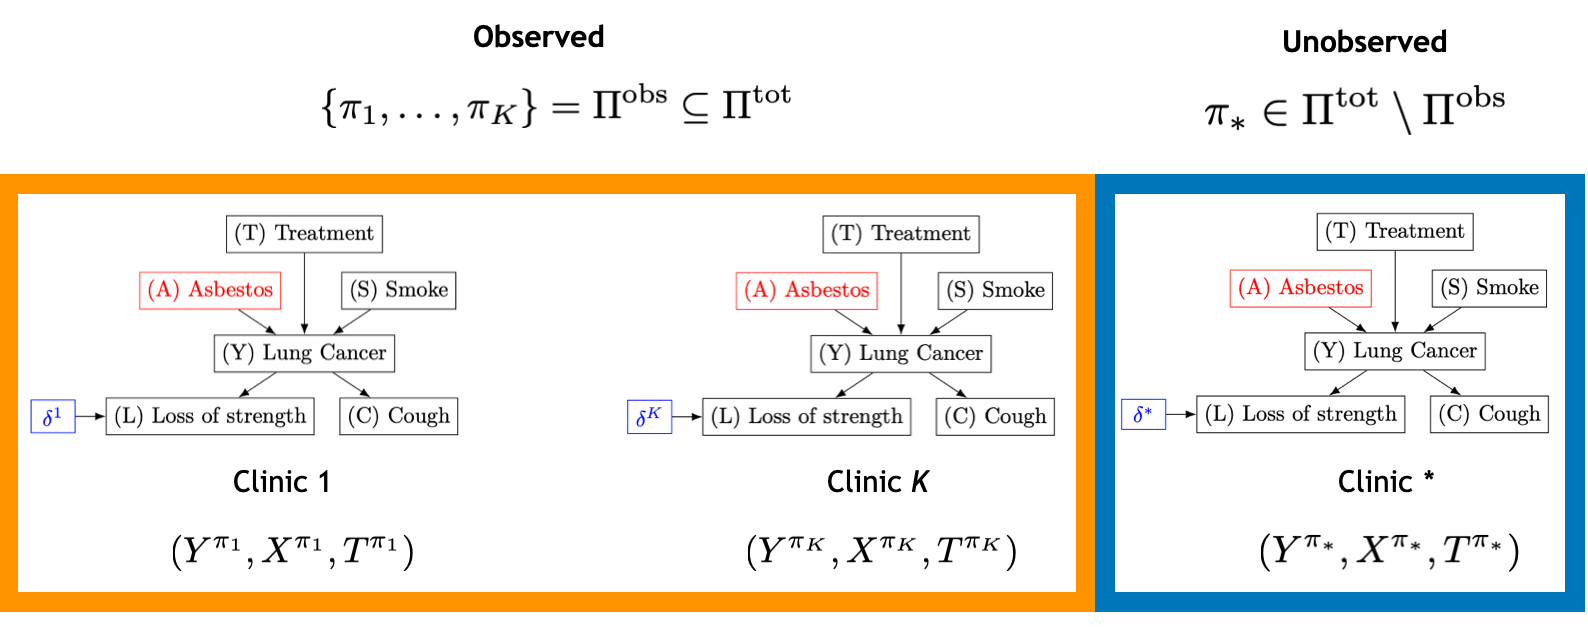
\includegraphics[width= 0.95\linewidth]{figures/illustration.png}
\end{figure}

\vskip-10pt

\small{

\begin{itemize}

\item We let $\delta^k, k=\{1, \ldots, K\},$ be a set of $K$  auxiliary variables which turn $G$ into an augmented graph $G_{\delta}$.

\item An edge $\delta^k \rightarrow X$ denotes a change in the causal mechanism that generates $X$.

\item In this example, the causal mechanism for \emph{Loss of Strength} changes between environments:

\vskip-10pt

\begin{equation*}
P^{\pi_i}(\text{Loss of strength} | \text{Cancer}) \neq P^{\pi_j}(\text{Loss of strength} | \text{Cancer})~\forall i \neq j \in K. 
\end{equation*}

\end{itemize}
}


\end{frame}

%%%%Slide

\begin{frame}
[fragile]\frametitle{Illustration (cont'd)}

Suppose the augmented Causal Graphs $G_{\delta}$ above are induced by the following Structural Causal Model (SCM):

\vskip10pt

\small{

\begin{equation*}
\begin{align*}
A := &  N_{A} \\
S :=  &  N_{S} \\
Y :=  &  A + S + T + 1.5 \times A \times T + 0.5 \times S \times T + N_Y\\
L :=   & \delta \times Y +N_L\\
C :=  &  0.3 \times Y + N_C  \\
\delta^k, ~k=\{1, \ldots, K\} \sim &~\text{U}(0,1) \\
\delta^* \sim &~\text{U}(-1,1) \\
T \sim &~\text{Bernoulli}(0.5) \\
N_j \sim &~\mathcal{N}(0,1)
\end{align*}
\end{equation*}
}

\end{frame}

%%%%Slide

\begin{frame}
[fragile]\frametitle{Illustration (cont'd)}

\begin{columns}[T] % align columns
\begin{column}{.48\textwidth}

\begin{center}
In-Distribution ($\Pi^{\text{obs}}$)
\end{center}

\vskip-17pt

\begin{figure}
   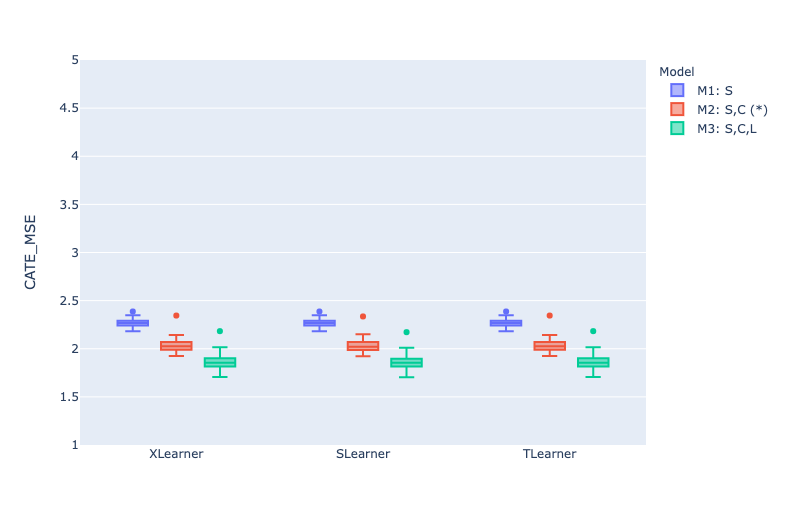
\includegraphics[width= 1.\linewidth]{figures/box1.png}
\end{figure}

\end{column}%
\hfill%
\begin{column}{.48\textwidth}
\begin{center}
Out-of-Distribution ($\pi_{*} \in \Pi^{\text{tot}} \setminus  \Pi^{\text{obs}}$)
\end{center}

\vskip-17pt

\begin{figure}
   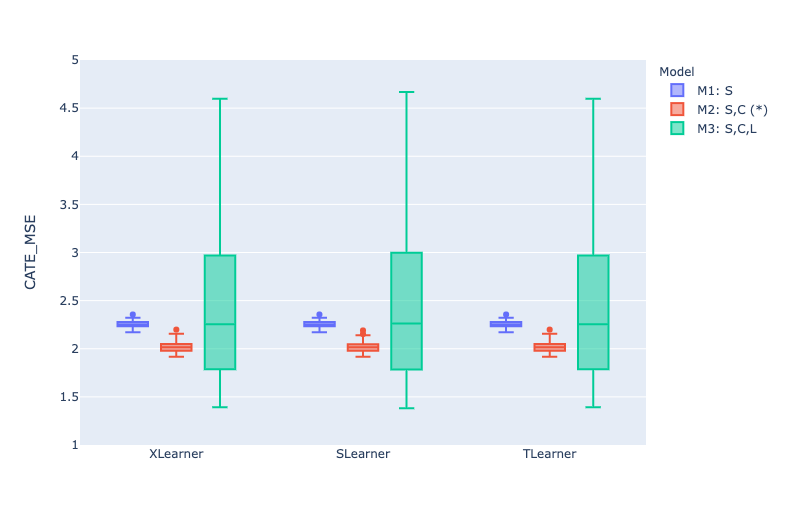
\includegraphics[width= 1.\linewidth]{figures/box2.png}
\end{figure}

\end{column}%
\end{columns}


\begin{itemize}

\item Inclusion of \emph{Cough} $(C)$ is beneficial for generalization performance.

\item Inclusion of \emph{Loss of Strength} $(L)$ is harmful for OOD generalization performance.


\item Our proposed approach selects \emph{Smoke} $(S)$ and \emph{Cough} $(C)$ as input features in CATE estimation (\textbf{Model 2}).

\end{itemize}


\end{frame}

%%%%Slide

\begin{frame}
[fragile]\frametitle{Key Challenges for Building Robust CATE Estimators}

\begin{itemize}

\item Recall the goal is to build a CATE estimator $\hat{\tau}(x)$ that minimizes the expected loss

\begin{equation}\label{objective}
\mathbb{E}_{(Y^{\pi_*}, X^{\pi_*}, T^{\pi_*}) \sim P^{\pi_*}} \ell(\hat{\tau}(x)},\tau})},
\end{equation}

\noindent based on experimental data from the source environments $\Pi^{\text{obs}}$.

\vskip10pt

\item We have two problems with~\ref{objective}:

\begin{enumerate}

\item No data from $P^{\pi_*}}$ are available at training time.

\item $\tau_i$ is not observed for an individual (due to the fundamental problem of causal inference).% This is the case for all environments $\pi \in \Pi^{\text{tot}}$ (not just for training environments  $\Pi^{\text{obs}},$ or test environment $\pi^*  \in \Pi^{\text{tot}} \setminus  \Pi^{\text{obs}}$).

\end{enumerate}

\end{itemize}



\end{frame}


%%%%Slide

\begin{frame}
[fragile]\frametitle{Invariant CATE Features}

\begin{definition}[Invariance]
A set of features $X^\mathrm{I},~\mathrm{I} \subseteq \{1, \ldots, p\}$, for estimating the CATE $P(y|do(t), x)$ from $\Pi^{\text{obs}}$ is invariant if for all $\pi_i, \pi_j \in \Pi^{\text{obs}}$ and for all $x \in \mathbb{X}$
\begin{equation*}
P^{\pi_i}(y|do(t), x^\mathrm{I}) = P^{\pi_j}(y|do(t), x^\mathrm{I}).
\end{equation*}
\end{definition}


\vskip10pt

Invariant sets are not unique. We let $\Omega$ be the collection of invariant CATE feature sets. 


\end{frame}



%%%%Slide

\begin{frame}
[fragile]\frametitle{Proposed CATE Estimator}

\textbf{Assumptions} \\

\vskip7pt

\textbf{A1.} There exists an invariant set of CATE features $X^\mathrm{I}$ (i.e., satisfying the invariance property defined above). \\

\vskip5pt

\textbf{A2.} The invariance property also hold for unseen environments $\pi^*  \in \Pi^{\text{tot}} \setminus  \Pi^{\text{obs}}$. \\

\vskip5pt

\textbf{A3.}  The conditional distribution $P(y|do(t), x)$ is linear (this addresses potential issues with non-overlapping feature supports). 


\vskip10pt

We propose linear CATE estimators $\hat{\tau}(x^{\mathrm{I}*};\mathbf{\theta})=\theta'x^{\mathrm{I}*},$ using an invariant set of features $X^{\mathrm{I}*} \in~\Omega$, identified from $\Pi^{\text{obs}}$.


\vskip10pt

Specifically, our proposed estimator with squared-error loss is given by 

\begin{equation*}
\theta^*{(x^\mathrm{I*})} =  \arg \min_{\theta} \frac{1}{\big| \mathcal{V} \big| } \sum_{i \in | \mathcal{V} |} \Big(  \hat{\tau_i}(x^\mathrm{I};\mathbf{\theta}) -  \check{\tau_i}  \Big)^2~~\forall  ~x^\mathrm{I} \in \Omega,
\end{equation*}

\noindent where $\check{\tau}_i$ is a plug-in estimate of $\tau_i$ estimated using data from a validation set $ \mathcal{V}$ \href{https://arxiv.org/pdf/1804.05146.pdf}{(Shuler et al., 2018)}. This attempts to circumvent the issue of unobserved $\tau$.

\end{frame}



%%%%Slide

\begin{frame}
[fragile]\frametitle{Robustness}

\small{

\begin{theorem}[Adversarial\footnote{Adapted from Rojas-Carulla et al. (2018).}]
Consider $(Y^{\pi_1}, X^{\pi_1}, T^{\pi_1}) \sim~P^{\pi_1},  \ldots,  (Y^{\pi_K}, X^{\pi_K}, T^{\pi_K}) \sim~P^{\pi_K}$ and an invariant set of CATE features $\mathrm{I}{*}$ satisfying \text{A1-A3}. The proposed estimator satisfies the following optimality statement over a set of distributions:

\begin{equation*}
\theta^*(\mathrm{I}{*}) \in  \arg \min_{\theta} \sup_{P^{\pi_*} \in \mathcal{P}} \mathbb{E}_{(Y^{\pi_*}, X^{\pi_*}, T^{\pi_*}) \sim P^{\pi_*}} \ell \Big(\hat{\tau}(x; \theta)},\check{\tau}}\Big)}.
\end{equation*}
\end{theorem}

\vskip10pt

Here $\mathcal{P}$ represents a family of distributions composed of all interventions on any subset of variables excluding $Y$.

}


\end{frame}


%%%%Slide

\begin{frame}
[fragile]\frametitle{Learning Invariant CATE Features}

\footnotesize{

\begin{algorithm}[H]

\scriptsize

\caption{Invariant CATE Features}
\label{A:ccifalg}

\textbf{Inputs:} Samples $(y_i^{\pi_k}, x_i^{\pi_k}, t_i^{\pi_k})_{i=1}^{n_k}$ from each environment $\pi_k, k \in \{1, \ldots, K\}$, and threshold $\alpha^c$ for independent test. \\ 
\textbf{Output:} Estimated invariant CATE feature set $X^\mathrm{I*}$. 
 
\begin{algorithmic}[1]


\STATE Set MSE=$[~]$, $\mathrm{I}=[~]$.

\STATE Create pseudo-outcome $W=2YT$ with $T = \pm  1$. (See \href{https://www.jstor.org/stable/24247388}{Tian et al., 2014}).

\FOR {$\mathrm{I} \subseteq \{1, \ldots, p\}$}

\STATE Linearly regress $W$ on $X^\mathrm{I}$  and compute the residuals $R_{\theta}^{k} = W^k - \theta'X^k$, $k \in \{1, \ldots, K\}$ on a validation set $\mathcal{V}$.

\STATE Test for equality in distributions of residuals across environments 

\begin{equation*}
H_0 = R_{\theta}^1\myeq R_{\theta}^2\myeq \ldots \myeq R_{\theta}^K,
\end{equation*}

and the corresponding p-value $\alpha$.

\IF {$\alpha > \alpha^c$}

\STATE Compute $\hat{\ell}_{\theta} = \frac{1}{\big| \mathcal{V} \big| } \sum_{i \in | \mathcal{V} |} \big(  \hat{\tau}(x^\mathrm{I};\mathbf{\theta}) -  \check{\tau} \big)^2$.

\STATE $\mathrm{I}$.append$(X^\mathrm{I})$, MSE.append$(\hat{\ell}_{\theta})$.

\ENDIF

\ENDFOR

\STATE Set $X^\mathrm{I*} = \mathrm{I}[ \arg \min \text{[MSE]} ]$.

\end{algorithmic}
\end{algorithm}

}
 
\end{frame}



%%%%Slide

\begin{frame}
[fragile]\frametitle{Numerical Experiments}

\begin{columns}[T] % align columns
\begin{column}{.40\textwidth}

\begin{figure}
   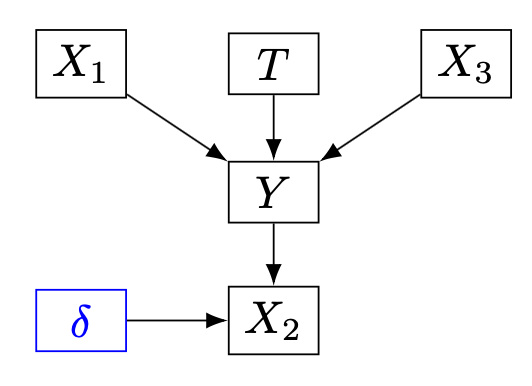
\includegraphics[width= 0.80\linewidth]{figures/SCM_experiment.png}
\end{figure}

\end{column}%
\hfill%
\begin{column}{.60\textwidth}


\small{
\begin{equation*}
\begin{align*}
X_1, X_3 \sim &  N(0,1) \\
Y :=  &  \alpha_1 X_1 + \alpha_2 X_3 + \alpha_3 T + \alpha_4 X_1\times T + \\
& \alpha_5 X_3 \times T + N_Y \\ 
X_2 := & \delta_k Y + N_{X_2} \\
N_Y \sim & N(0, 1.5) \\
\delta^k,  \delta* \sim &~\text{U}(0,1),~k=\{1, \ldots, K\} \\
 N_{X_2} \sim & N(0,0.1) \\ 
 \alpha_1, \ldots, \alpha_5 \sim & \text{U}(-1,2.5) \\
\end{align*}
\end{equation*}
}



\end{column}%
\end{columns}


\end{frame}



%%%%Slide

\begin{frame}
[fragile]\frametitle{Numerical Experiments: Results}

\footnotesize{
\begin {table}[H]
\caption {CATE MSE: Mean and (SE)} \label{tab:title} 
\begin{center}
\begin{tabular}{LSSSSS} \toprule
 {Pool Method}\\ \midrule
    {$N$} & {$K=3$} & {$K=6$} & {$K=10$} & {$K=15$} & {$K=20$}  \\ \midrule
   
    200 &   \textcolor{blue}{2.107} & \textcolor{blue}{1.588} & \textcolor{blue}{1.391} & \textcolor{blue}{1.298} & \textcolor{blue}{1.025} \\
           &  {(0.419)}& {(0.379)}& {(0.378)}& {(0.330)}& {(0.245)}\\
    400 &  \textcolor{blue}{1.807} & \text{1.222} & \text{0.935} & \text{1.109} & \text{1.140}  \\
          &  {(0.345)}& {(0.179)}& {(0.120)}& {(0.159)}& {(0.196)} \\
    800 & \textcolor{blue}{1.535} & \text{1.461} & \text{0.958} & \text{1.445} & \text{1.152} \\
         & {(0.203)}& {(0.234)}& {(0.133)}& {(0.334)}& {(0.331)} \\
 1200 & \text{1.385} & \text{1.438} & \text{1.222} & \text{1.047} & \text{0.924} \\ 
         & {(0.233)}& {(0.414)}& {(0.223)}& {(0.158)}& {(0.143)} \\ \midrule
 
   
    {Proposed Method}  \\ \midrule
    200 & \text{4.502} & \text{1.932}& \text{1.864}& \text{2.144} & \text{1.552} \\ 
&  {(2.078)}& {(0.484)}& {(0.473)}& {(0.542)}& {(0.473)}\\ 
    400 &  \text{1.851} & \textcolor{blue}{0.598} & \textcolor{blue}{0.573} & \textcolor{blue}{0.490} & \textcolor{blue}{0.206}\\ 
&  {(0.712)}& {(0.278)}& {(0.194)}& {(0.211)}& {(0.116)} \\
    800 &  \text{1.618} & \textcolor{blue}{0.538} & \textcolor{blue}{0.142} & \textcolor{blue}{0.077} & \textcolor{blue}{0.073} \\ 
&  {(0.536)}& {(0.296)}& {(0.094)}& {(0.049)}& {(0.051)} \\
 1200 & \textcolor{blue}{ 0.113} & \textcolor{blue}{0.059} & \textcolor{blue}{0.258} & \textcolor{blue}{0.102} & \textcolor{blue}{0.003} \\ 
 & {(0.076)}& {(0.042)}& {(0.162)}& {(0.070)}& {(0.002)} \\\toprule

\end{tabular}
\end{center}
\end {table}
}


\end{frame}


%%%%Slide

\begin{frame}
[fragile]\frametitle{Takeaways}

\begin{itemize}

\item We relax the i.i.d. assumption from CATE estimation methods.

\item We  propose a method to select CATE models that are robust under a family of distributional changes in the data.

\item The proposed method shows positive results on a limited number of simulation scenarios.


\end{itemize}



\end{frame}




\end{document}

